\documentclass[tikz,border=6pt]{standalone}
\usepackage{amsmath,amssymb}
\usepackage{xcolor}
\definecolor{accent}{HTML}{A13D2C}
\definecolor{accent2}{HTML}{2B5F6B}
\definecolor{muted}{HTML}{5A564F}
\definecolor{linecol}{HTML}{D8D2C4}
\definecolor{astroblue}{HTML}{1B4F72}
\usetikzlibrary{arrows.meta}
\usepackage[T1]{fontenc}\usepackage{newpxtext,newpxmath}  % same fonts as the notes
\begin{document}
% Grey atmosphere in the Eddington approximation: T/T_eff = [ (3/4)(tau + 2/3) ]^(1/4).
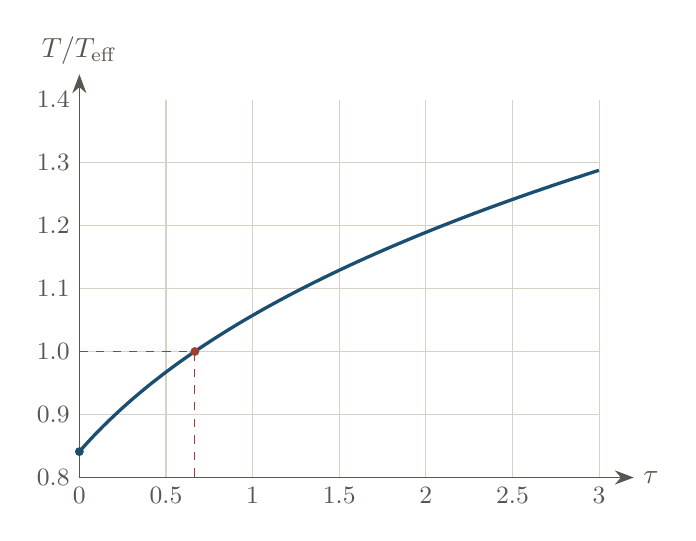
\begin{tikzpicture}[x=2.2cm,y=8cm, >={Stealth[length=2.4mm]}]
  \draw[linecol] (0,0.8) grid[xstep=0.5,ystep=0.1] (3,1.4);
  \draw[->, muted] (0,0.8) -- (3.2,0.8) node[right] {$\tau$};
  \draw[->, muted] (0,0.8) -- (0,1.44) node[above] {$T/T_{\rm eff}$};
  \foreach \x in {0,0.5,1,1.5,2,2.5,3} \node[below, muted] at (\x,0.8) {\small \x};
  \foreach \y in {0.8,0.9,1.0,1.1,1.2,1.3,1.4} \node[left, muted] at (0,\y) {\small \y};
  \draw[astroblue, line width=1.2pt, domain=0:3, samples=150] plot (\x, {(0.75*(\x+2/3))^(0.25)});
  \draw[dashed, accent] (0,1) -- (2/3,1) -- (2/3,0.8);
  \fill[accent] (2/3,1) circle (1.6pt);
  \fill[astroblue] (0,{(0.5)^(0.25)}) circle (1.6pt);
\end{tikzpicture}
\end{document}
